\setlength{\columnsep}{3pt}
\begin{flushleft}
	\bigskip
	An array is \textbf{indexed collection of fixed number of homogeneous data elements}.
	
	\bigskip\bigskip
	\begin{figure}[h!]
		\centering
		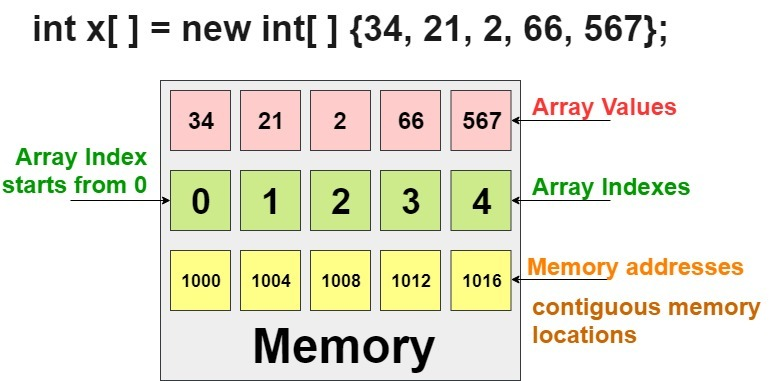
\includegraphics[scale=.45]{content/chapter4/images/array.jpg}
	\end{figure}		
	
	\textbf{Advantage}:
	\begin{itemize}
		\item Array can represent huge number of values using single variable that will improve readability of code.
	\end{itemize}
	
	\textbf{Disadvantage}:
	\begin{itemize}
		\item Array are fixed in size.
		\item Once an array is created, they cannot be increased or decreased.
		\item Array size need to be mentioned in advance, which is not always possible.
	\end{itemize}
	
	
\end{flushleft}




